\documentclass{article}
%\usepackage[utf8]{inputenc}
\usepackage[utf8]{vietnam}
\usepackage{amsmath,amsxtra,amssymb,latexsym, amscd,amsthm}
\usepackage{mathtools}
\usepackage{graphicx}
\usepackage{wrapfig}
\usepackage{blindtext}
\usepackage{csquotes}


\newcommand{\norm}[1]{\left\lVert#1\right\rVert}
\newcommand{\twonorm}[1]{\left\lVert#1\right\rVert_{2}}

\title{$p\,$-norm of matrices}
\author{phunc20}
\date{\today}


\begin{document}
\theoremstyle{definition}
\newtheorem{Spiel}{Vd}[section]


\maketitle
\section{Động cơ}
%Tại sao người ta lại nghĩ đến định nghĩa $\Vert A \Vert := \sup_{\bold{x} \ne \bold{0}} \frac{A\bold{x}}{\Vert \bold{x} \Vert}$
%Tại sao người ta lại nghĩ đến định nghĩa $\Vert A \Vert \mathrel{\mathop:}= \sup_{\bold{x} \ne \bold{0}} \frac{A\bold{x}}{\Vert \bold{x} \Vert}$
%Tại sao người ta lại nghĩ đến định nghĩa $\Vert A \Vert \coloneqq \sup_{\bold{x} \ne \bold{0}} \frac{A\bold{x}}{\Vert \bold{x} \Vert}$
Tại sao người ta lại nghĩ đến định nghĩa norm của một ma trận $A \in M_{m,n}(\mathbb{C})$
$$\norm{A} \,\,\coloneqq\!\! \sup_{\mathbf{x} \,\in\, {\mathbb{C}^{n} \setminus \{\mathbf{0}\}}} \frac{\norm{A\mathbf{x}}}{\norm{\mathbf{x}}}\;$$
như thế này?

\textbf{Rmk.} Why we choose to not specify exactly which norm above?

\textbf{Rmk2.} Cho dù mình viết $\mathbb{C}^n$ bạn đọc cũng có thể suy nghĩ trong $\mathbb{R}^n$.

\section{Ý tưởng}
Bây giờ giả bộ như chúng ta không biết về sự tồn tại của định nghĩa này, và chúng ta cùng đi tìm một định nghĩa hợp lý
cho norm của một ma trận. Các norm $\norm{A\mathbf{x}}$ va $\norm{\mathbf{x}}$ đã được định nghĩa rõ rằng, lúc này  mình sẽ tự hỏi
\begin{displayquote}
chúng ta có thể định nghĩa ra $\norm{A}$ sao cho $\norm{A\mathbf{x}} \stackrel{?}{=} \norm{A}\cdot\norm{\mathbf{x}}$ không?
\end{displayquote}

%Tiếp theo chúng ta sẽ đi kiểm ví dụ ngược/trốn lại cái đẳng thức ở trên. Nếu kiểm không được mình sẽ đi chứng minh nó.
Một counter-example có thể hướng dẫn chúng ta:
\begin{Spiel}
  %Consider the following matrix and vectors with the standard $2$-norm in $\mathbb{R}$\\
	Xét ma trận $A$ và vectơ $\mathbf{x_1}, \mathbf{x_2}$ như sau
  $$
    A = \begin{pmatrix}
    	3 &  5 \\
    	4 & 12 \\
    \end{pmatrix},\;
    \mathbf{x_1} = \begin{pmatrix} 1 \\ 0 \end{pmatrix},\;
    \mathbf{x_2} = \begin{pmatrix} 0 \\ 1 \end{pmatrix}.
  $$
  %with the standard $2$-norm in $\mathbb{R}$
  Với cái $2$-norm quen thuộc trong $\mathbb{R}^2$, chúng ta có
  $$
	  \begin{aligned}
			%% Cannot \small neither \tiny in math mode
			%\norm{\mathbf{x_1}}_{\small 2} = 1, \twonorm{\mathbf{x_2}} = 1
			%\norm{\mathbf{x_1}}_{\tiny 2} = 1, \twonorm{\mathbf{x_2}} = 1
			%& \norm{\mathbf{x_1}}_{2} = 1,\; \twonorm{\mathbf{x_2}} = 1, \\
			& \norm{\mathbf{x_1}}_{2} = 1,\; \twonorm{\mathbf{x_2}} = 1, \nonumber \\
			& \norm{A \mathbf{x_1}}_{2} = \norm{\begin{pmatrix} 3 \\ 4 \end{pmatrix}}_{2} = 5, \\
			%& \begin{equation}
			%	  \norm{A \mathbf{x_1}}_{2} = \norm{\begin{pmatrix} 3 \\ 4 \end{pmatrix}}_{2} = 5,
      %  \end{equation} \\
			& \norm{A \mathbf{x_2}}_{2} = \norm{\begin{pmatrix} 5 \\ 12 \end{pmatrix}}_{2} = 13. \\
	  \end{aligned}
  $$
	Từ ví dụ này chúng ta có thể nhìn ra $\norm{A\mathbf{x}} \stackrel{?}{=} \norm{A}\cdot\norm{\mathbf{x}}$ \textbf{không khá thi}. Bởi vì nếu như đẳng thức có thật, thì 
  $$
	  \begin{aligned}
			& \norm{A \mathbf{x_1}}_{2} = 5 \implies \norm{A}_{2} = 5 \\
			& \norm{A \mathbf{x_2}}_{2} = 13 \implies \norm{A}_{2} = 13 \\
			& \qquad\qquad\qquad \rightarrow\!\leftarrow
	  \end{aligned}
  $$
\end{Spiel}

Nếu vậy sẽ rất hợp lý cho chúng ta chuyển sang một mục tiêu yếu hơn, đó là
$$
  \begin{aligned}
    \norm{A\mathbf{x}} \stackrel{?}{\le} \norm{A}\cdot\norm{\mathbf{x}} \quad\forall\;\; \mathbf{x} \in \mathbb{C}^n \\
		\\
		\text{tương đương với} \\
		\\
		\norm{A} \stackrel{?}{\ge}  \frac{\norm{A\mathbf{x}}}{\norm{\mathbf{x}}}  \quad\forall\;\; \mathbf{x} \ne \mathbf{0}. \\
  \end{aligned}
$$
Chúng ta đã có thể nhận ra hình dáng của định nghĩa \textit{bí ấn} ban đầu.

Nhắc lại $\sup S$ của một tập $S \subset \mathbb{R}$ tiếng Anh được gọi là \textit{least upper bound}, tức là con số chặn trên nhỏ nhất.
Chúng ta dĩ nhiên sẽ hỏi:
Tập $\left\{\frac{\norm{A\mathbf{x}}}{\norm{\mathbf{x}}} \;|\; \mathbf{x} \in \mathbb{C}^n \setminus \mathbf{0}\right\}$ có bị chặn ở trên không?


\begin{wrapfigure}{p}{0.5\textwidth}
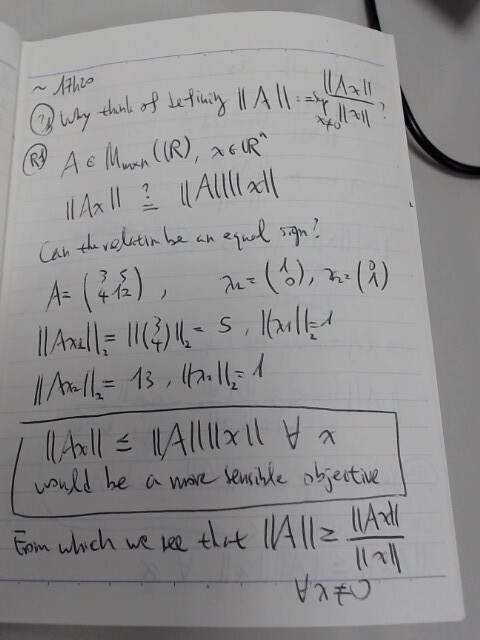
\includegraphics[width=0.4\textwidth]{01-motivation.jpg}
%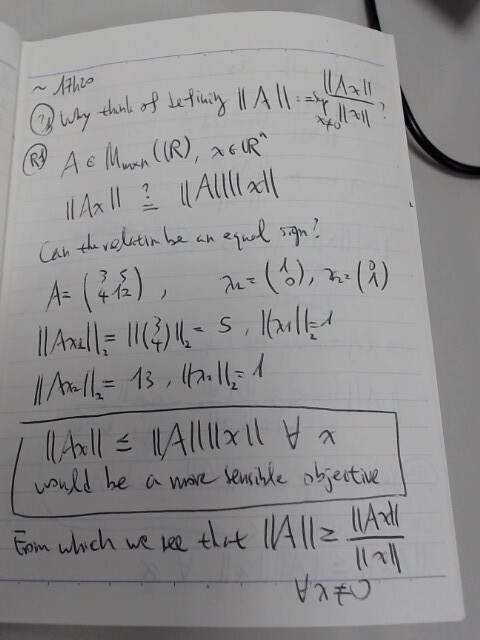
\includegraphics[width=2.5cm]{01-motivation.jpg}
%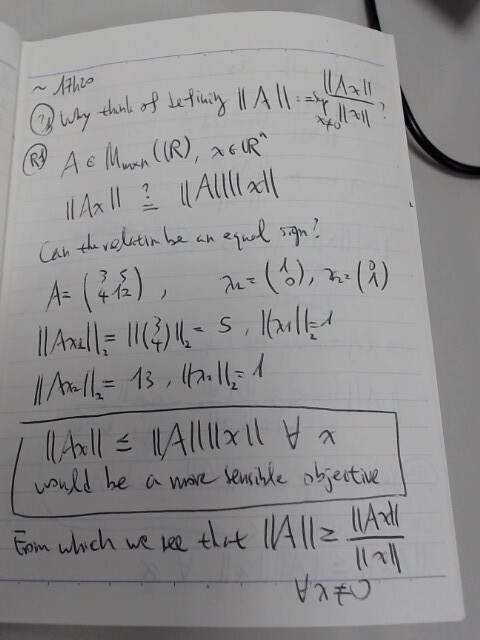
\includegraphics{01-motivation.jpg}
\end{wrapfigure}

\begin{wrapfigure}{h}{0.5\textwidth}
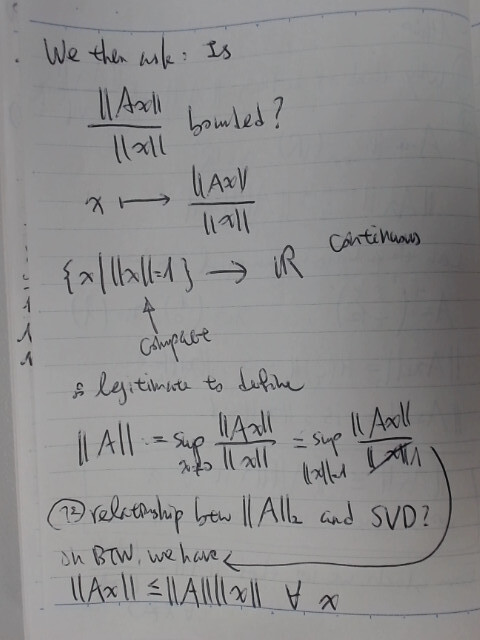
\includegraphics[width=0.4\textwidth]{02-moti_cont.jpg}
\end{wrapfigure}
\blindtext


\blindtext

%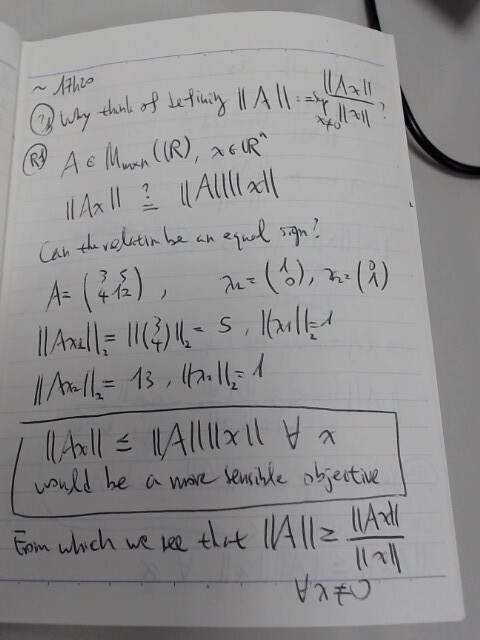
\includegraphics[width=0.7\textwidth]{01-motivation.jpg}
%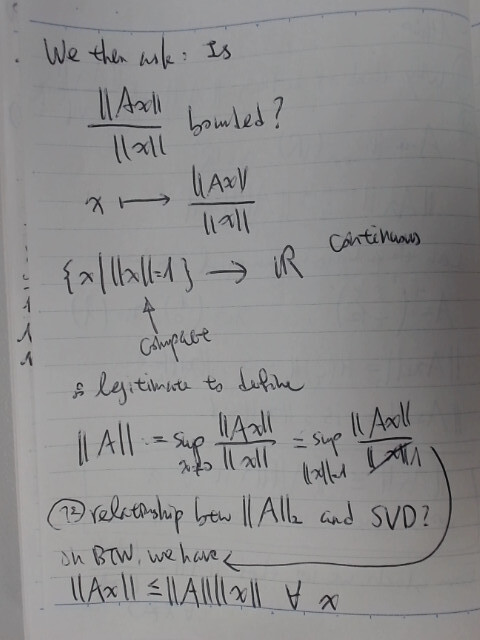
\includegraphics[width=0.7\textwidth]{02-moti_cont.jpg}
%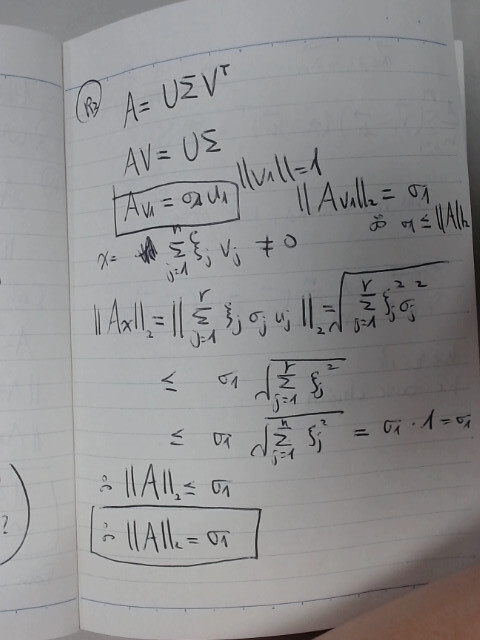
\includegraphics[width=0.7\textwidth]{03-2norm_and_singular_value.jpg}
%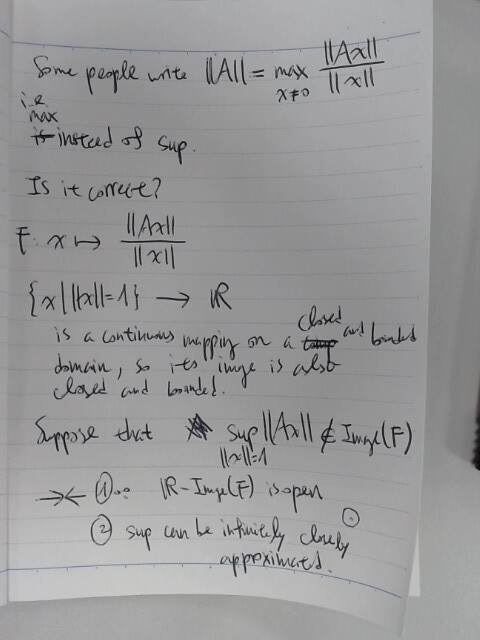
\includegraphics[width=0.7\textwidth]{04-max_instead.jpg}

\end{document}





%   01-motivation.jpg
%   02-moti_cont.jpg
%   03-2norm_and_singular_value.jpg
%   04-max_instead.jpg
%   covariance.jpg
%   decompression.jpg
%   motivation.tex
%   vietnamese.tex

